\documentclass[a4paper,12pt]{article}
%\documentclass[a4paper,10pt]{scrartcl}

\usepackage[utf8x]{inputenc}
\usepackage{amsfonts}
\usepackage{amsmath,esint}
\usepackage{graphicx}
\usepackage{pdfpages}
\usepackage{sansmath}
\usepackage{hyperref}
\usepackage{natbib}

\definecolor{boiseBlue} {RGB}{29,72,159}
\definecolor{rojoAmor} {RGB}{171,13,4}
\definecolor{moradoAmor} {RGB}{93,8,113}
\definecolor{verdeAmor} {RGB}{98,158,31}
\definecolor{negro} {RGB}{10,10,10}
\definecolor{lgreen} {RGB}{180,210,100}
\definecolor{dblue}  {RGB}{20,66,129}
\definecolor{ddblue} {RGB}{11,36,69}
\definecolor{lred}   {RGB}{220,0,0}
\definecolor{nred}   {RGB}{224,0,0}
\definecolor{norange}{RGB}{230,120,20}
\definecolor{nyellow}{RGB}{255,221,0}
\definecolor{ngreen} {RGB}{98,158,31}
\definecolor{dgreen} {RGB}{78,138,21}
\definecolor{nblue}  {RGB}{28,130,185}
\definecolor{jblue}  {RGB}{20,50,100}

\usepackage{listings}
\usepackage{xcolor}
\lstset{language=C++,
		basicstyle=\ttfamily,
	       backgroundcolor=\color{black!5}\ttfamily,
                keywordstyle=\color{nblue}\ttfamily,
                stringstyle=\color{nred}\ttfamily,
                commentstyle=\color{ngreen}\ttfamily,
                morecomment=[l][\color{moradoAmor}]{\#}
}

\newenvironment{rcases}{\left.\begin{aligned}}{\end{aligned}\right\rbrace}

\renewcommand{\familydefault}{\sfdefault}

\newcommand{\specialcell}[2][c]{%
  \begin{tabular}[#1]{@{}c@{}}#2\end{tabular}}
% \specialcell{Foo\\bar}

\title{wave solver with PML \\ \small{summer 2017}}
\author{}
\date{}

\pdfinfo{%
  /Title    ()
  /Author   ()
  /Creator  ()
  /Producer ()
  /Subject  ()
  /Keywords ()
}

\begin{document}
\maketitle
%-------------------
% main flow
%-------------------
%\newpage
%\section{Main code flow}
\begin{figure}
\centering
\includegraphics[width=0.7\textwidth]{../pics/tikz/wave-flow.pdf}
\caption{Main code flow.}
\end{figure}
%-------------------
% set up
%-------------------
%\newpage
%\section{Setup}
%
\begin{figure}
\centering
\includegraphics[width=0.7\textwidth]{../pics/tikz/dx-dy-dt.pdf}
\caption{Calculation of $\Delta x, \Delta y$ and $\Delta t$.}
\end{figure}
%-------------------
% fields inner
%-------------------
%\newpage
%\section{Field updates (inner)}
%
\begin{figure}
\centering
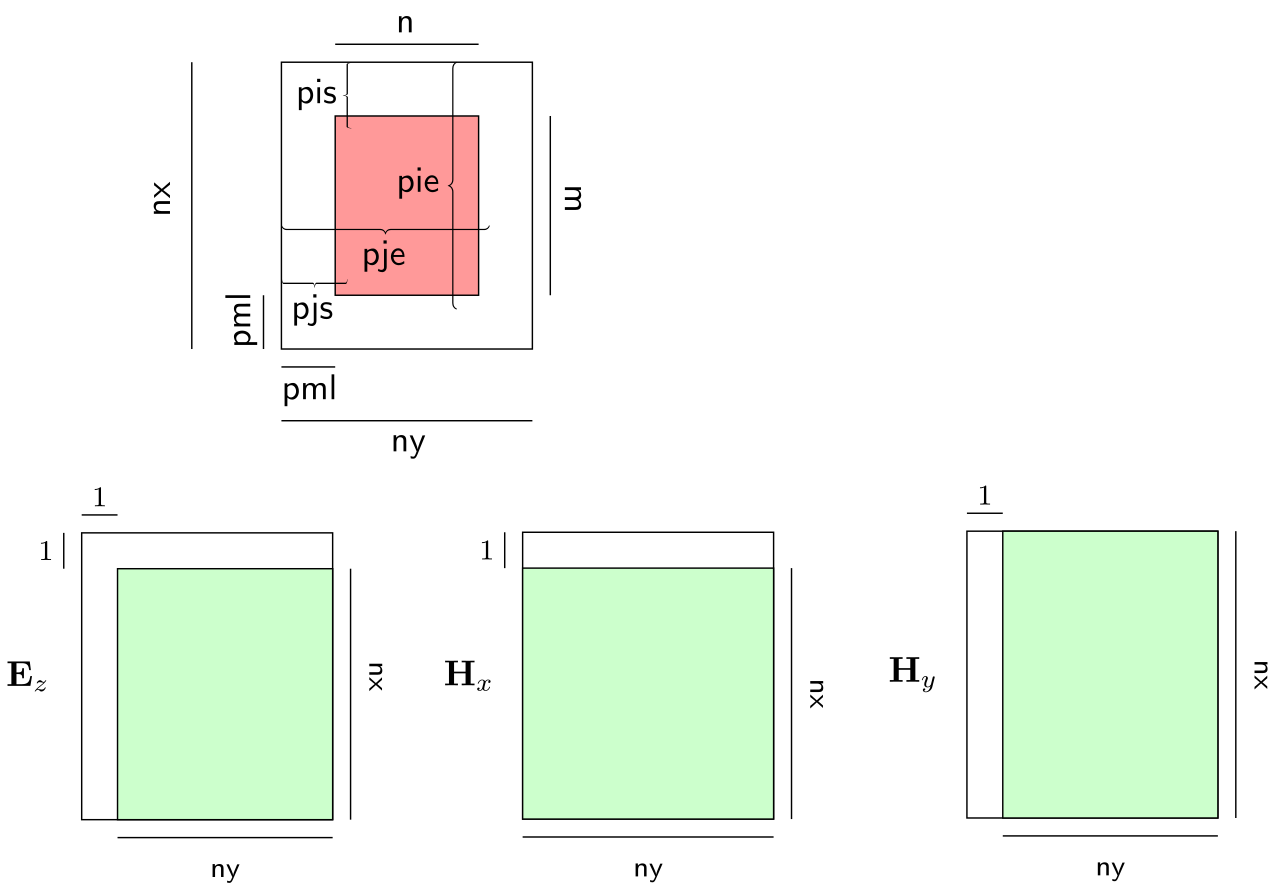
\includegraphics[width=1\textwidth]{../pics/tikz/svg/EzHxHy.pdf}
\caption{Grid dimensions of ${\bf E}_z,\; {\bf H}_x,\; {\bf H}_y$.}
\end{figure}
%
\begin{figure}
\centering
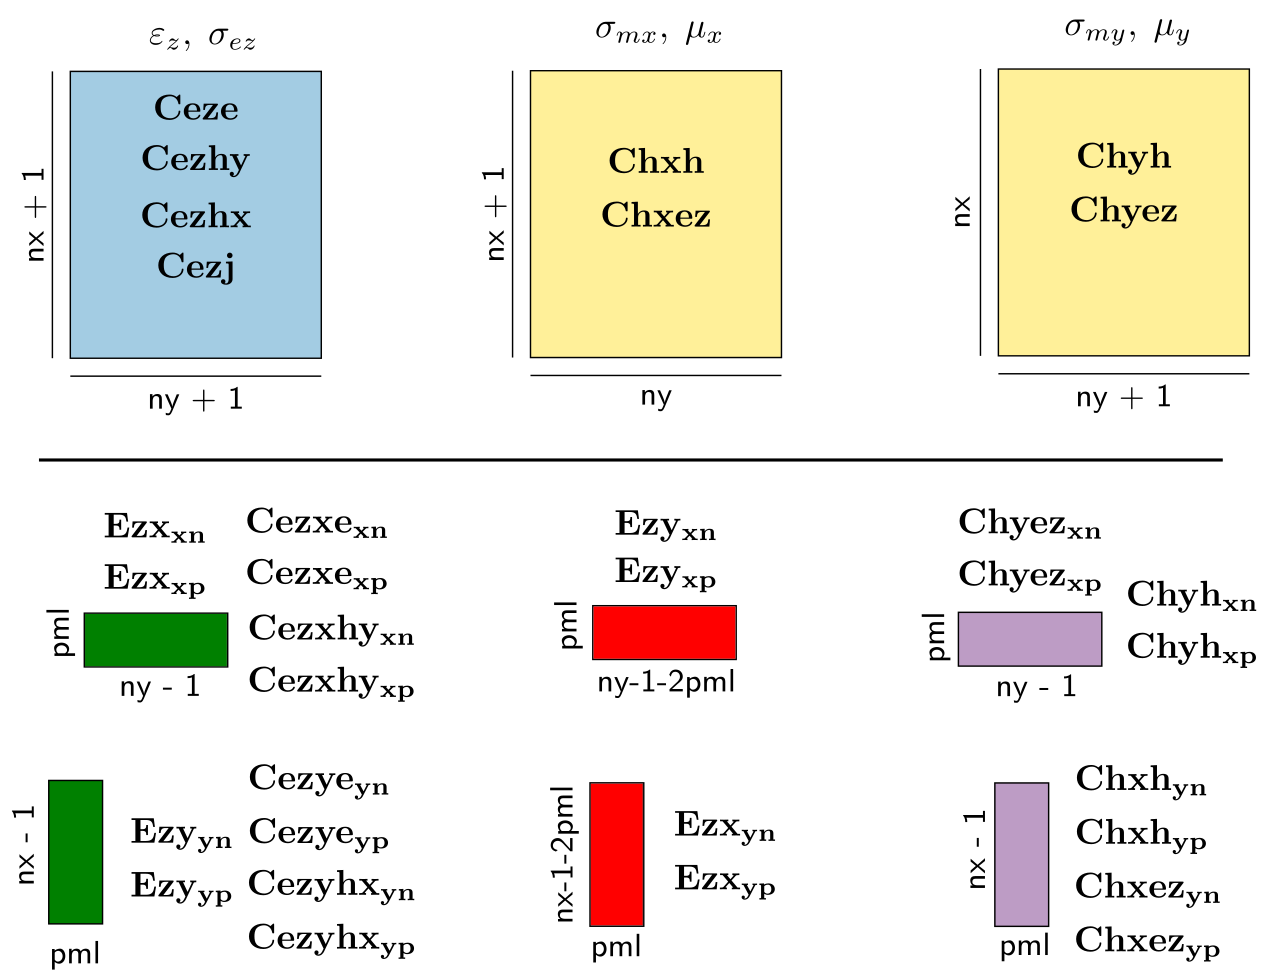
\includegraphics[width=1\textwidth]{../pics/tikz/svg/coeff.pdf}
\caption{Coefficients of all nodes ({\bf up}), and PML nodes ({\bf down}).}
\end{figure}
%
\begin{figure}
\centering
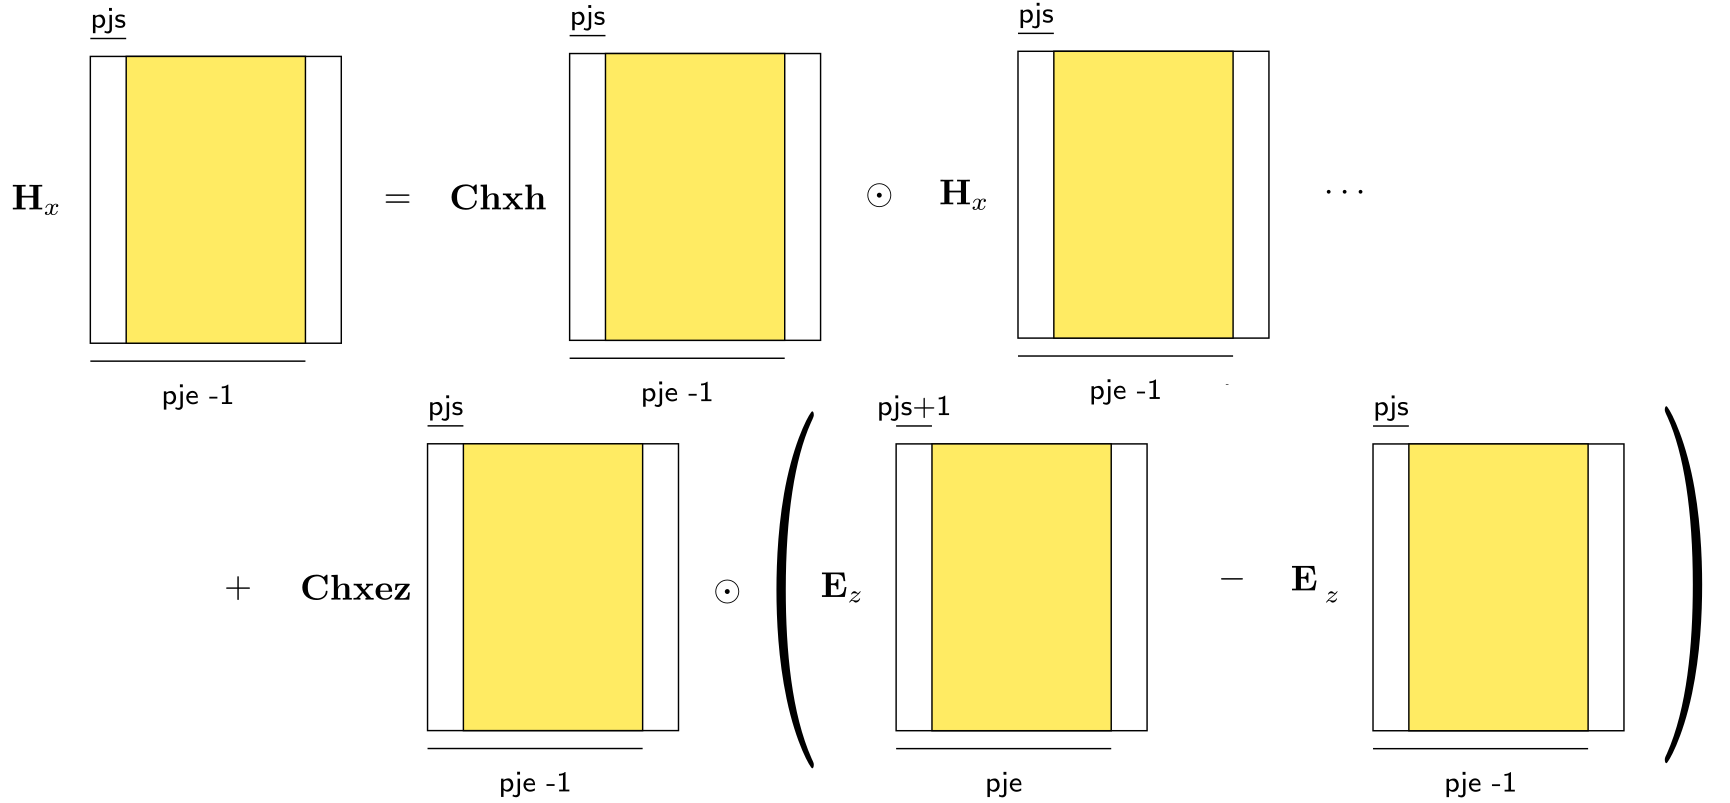
\includegraphics[width=1\textwidth]{../pics/tikz/svg/Hx-new-inside.pdf}
~
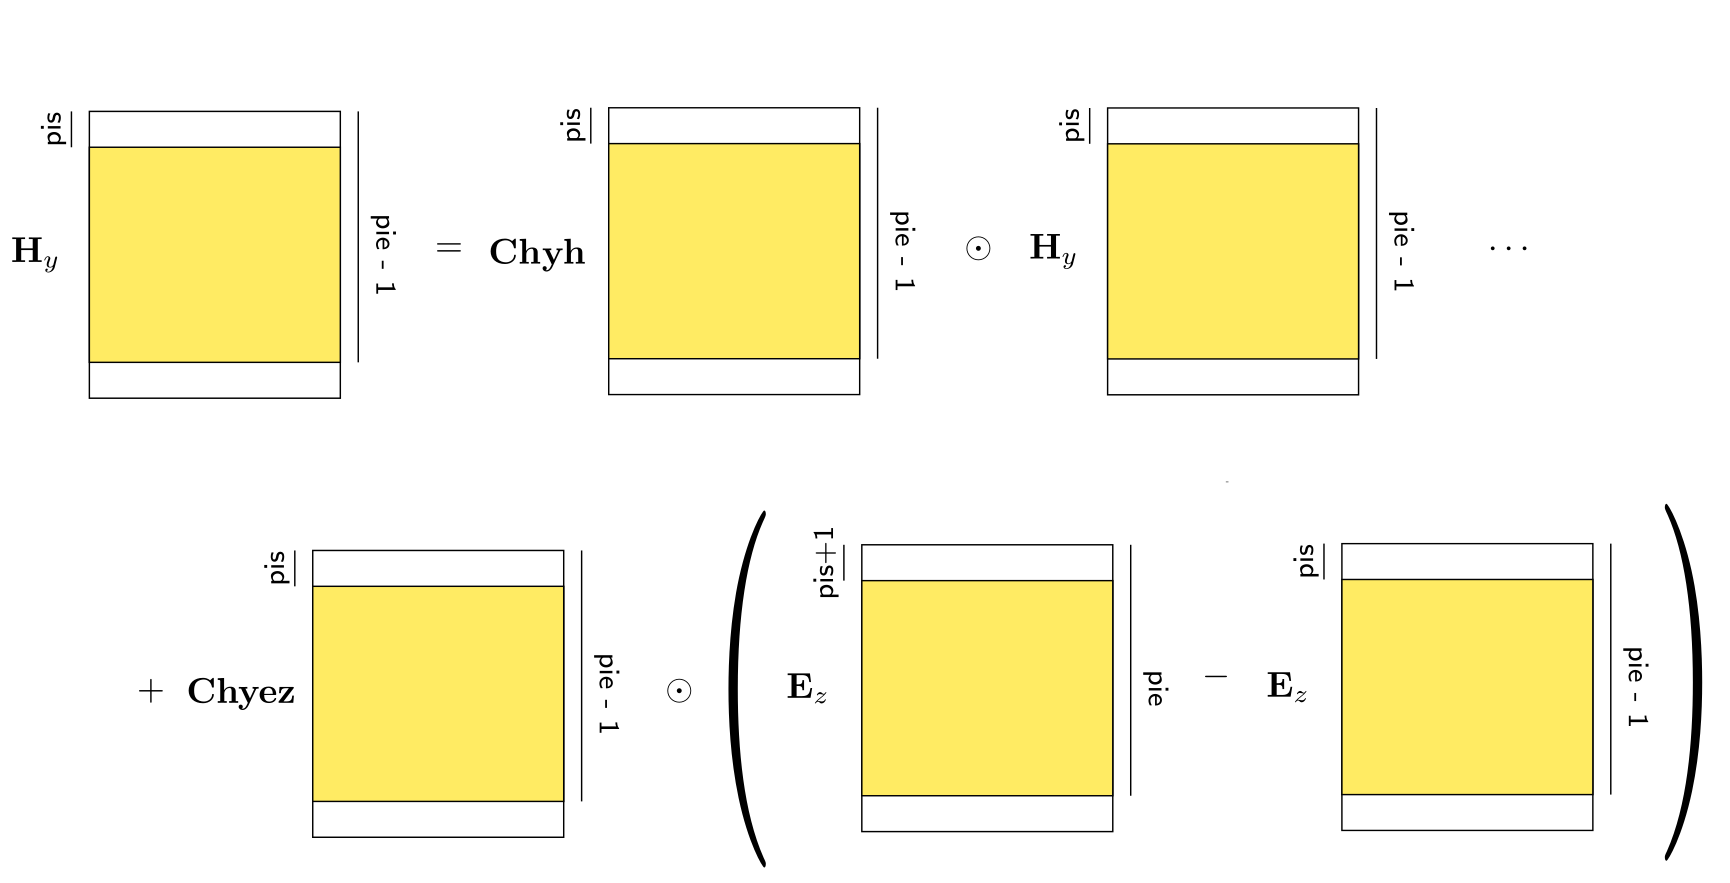
\includegraphics[width=1\textwidth]{../pics/tikz/svg/Hy-new-inside.pdf}
\caption{Update of ${\bf H}_x$ and ${\bf H}_y$. One line of nodes into PML.}
\end{figure}
%
\begin{figure}
\centering
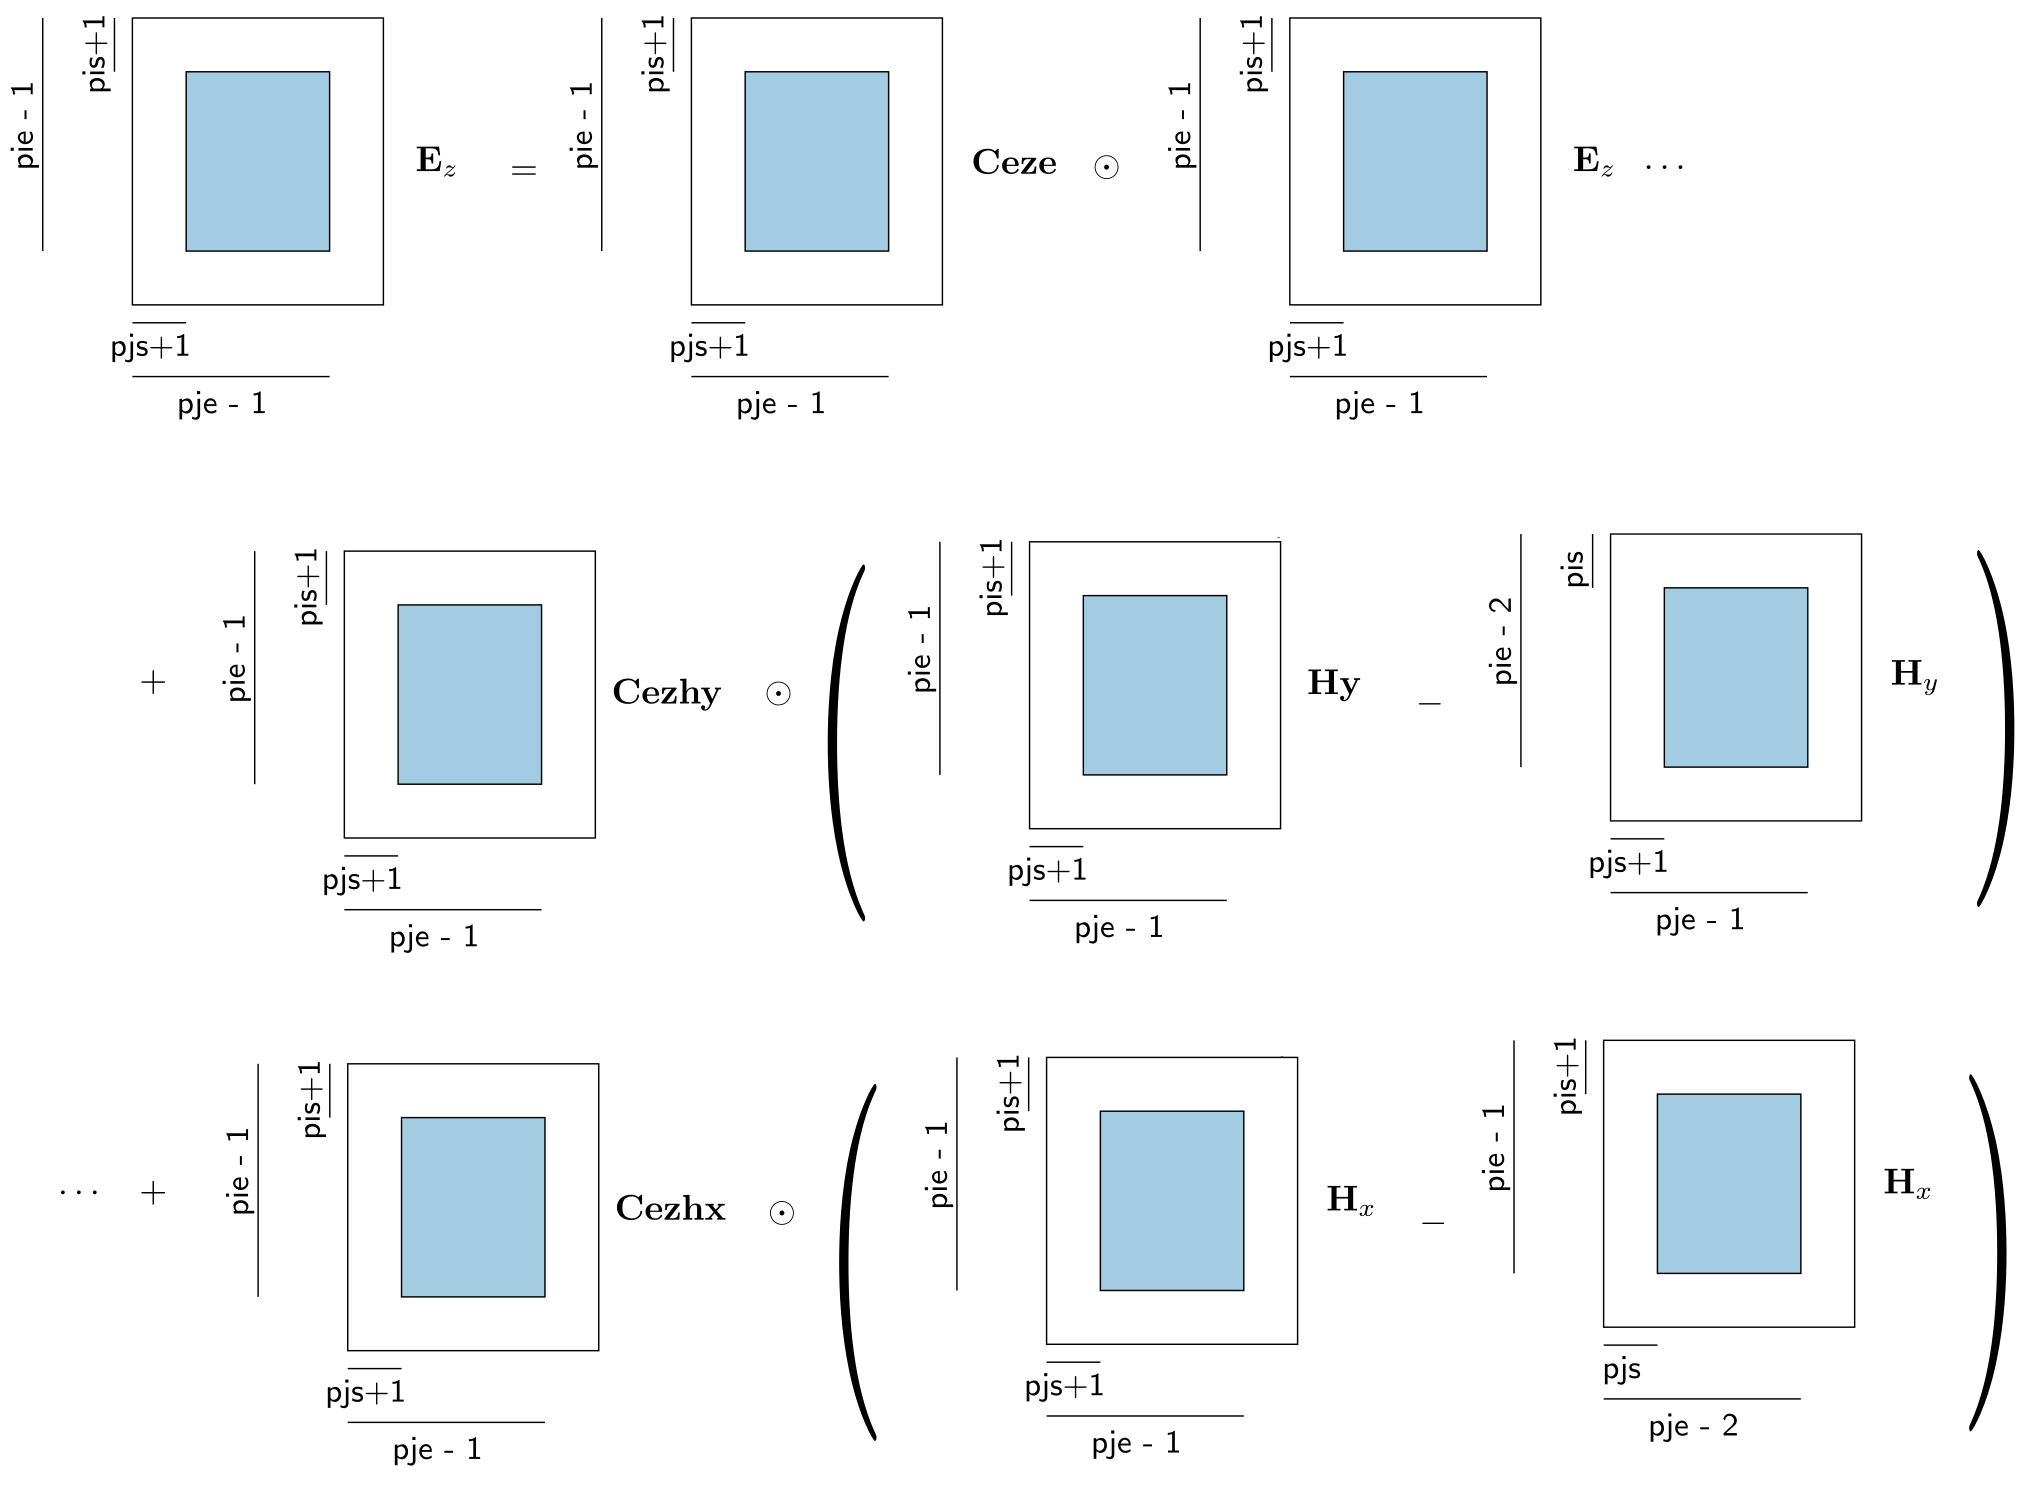
\includegraphics[width=1\textwidth]{../pics/tikz/svg/Ez-new-inside.pdf}
\caption{Update of ${\bf E}_z$. One line of nodes into PML.}
\end{figure}
%-------------------
% fields pml
%-------------------
%\newpage
%\section{Field updates (PML)}
%
%
\begin{figure}
\centering
\includegraphics[width=1\textwidth]{../pics/tikz/svg/pml-color/Hx-pml-yn.pdf}
~
\includegraphics[width=1\textwidth]{../pics/tikz/svg/pml-color/Hx-pml-yp.pdf}
\caption{PML update for ${\bf H}_x$. PML proper.}
\end{figure}
%
\begin{figure}
\centering
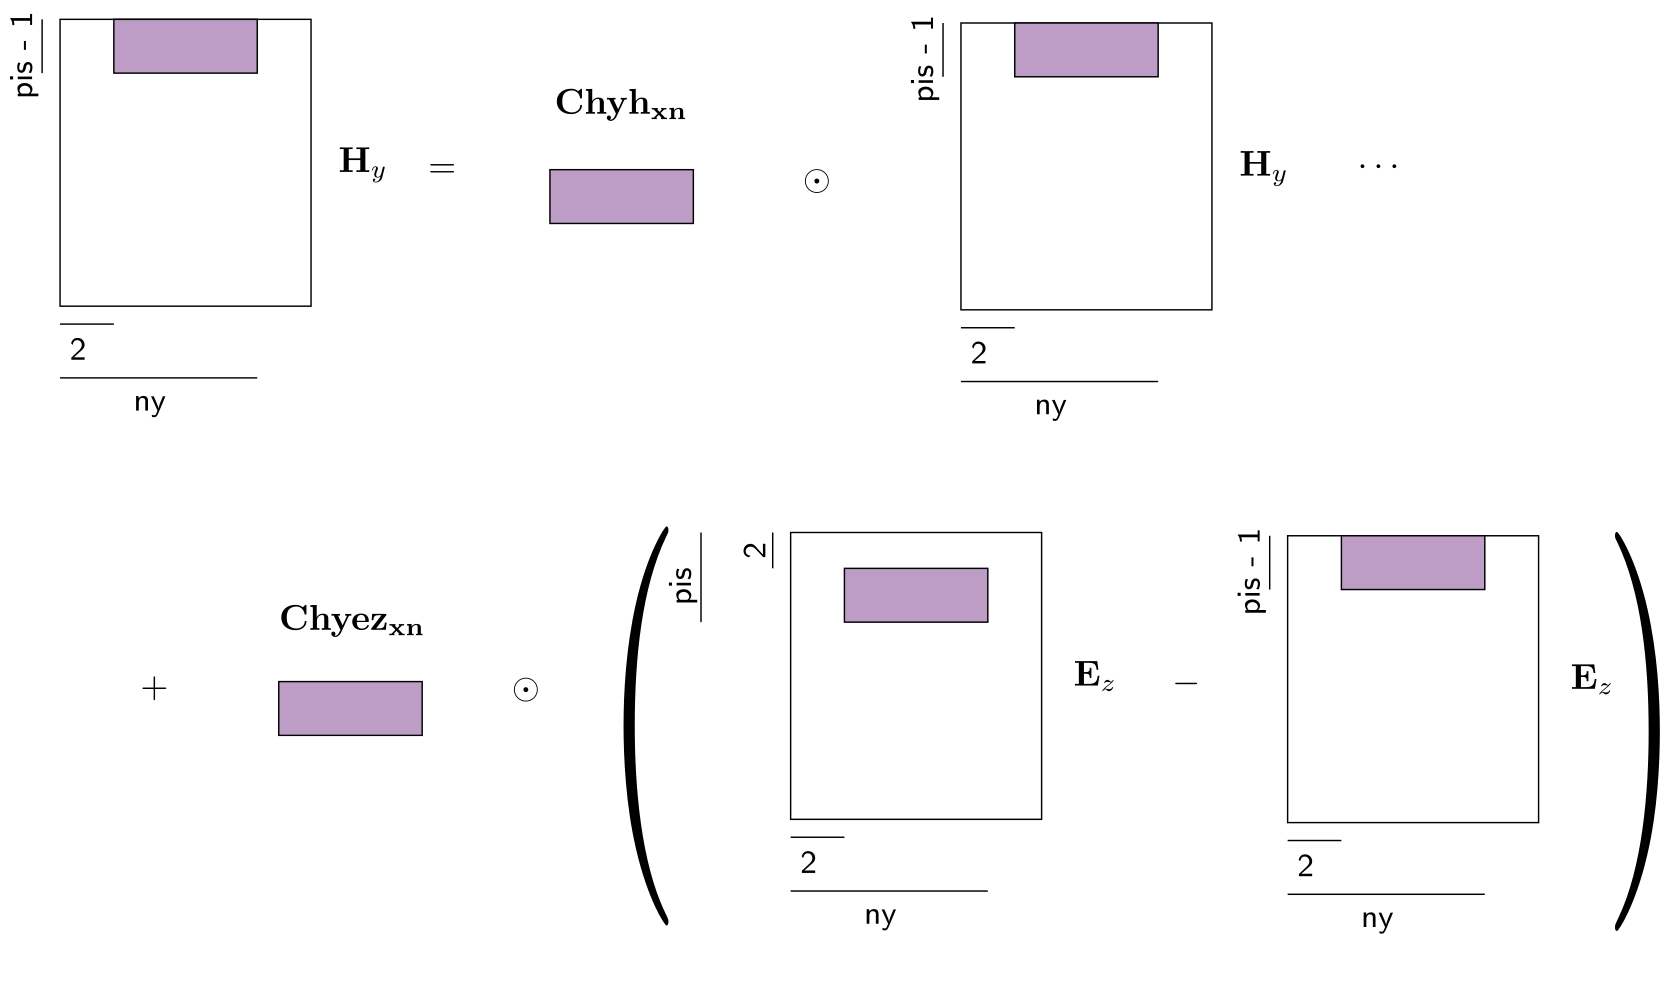
\includegraphics[width=1\textwidth]{../pics/tikz/svg/pml-color/Hy-pml-xn.pdf}
~
\includegraphics[width=1\textwidth]{../pics/tikz/svg/pml-color/Hy-pml-xp.pdf}
\caption{PML update for ${\bf H}_y$. PML proper.}
\end{figure}
%
%
\begin{figure}
\centering
\includegraphics[width=1\textwidth]{../pics/tikz/svg/pml-color/Ezx-xn.pdf}
~
\includegraphics[width=1\textwidth]{../pics/tikz/svg/pml-color/Ezy-xn.pdf}
\caption{PML update for ${\bf E}_{zx}$ up. One line of nodes into inner nodes.}
\end{figure}
%
\begin{figure}
\centering
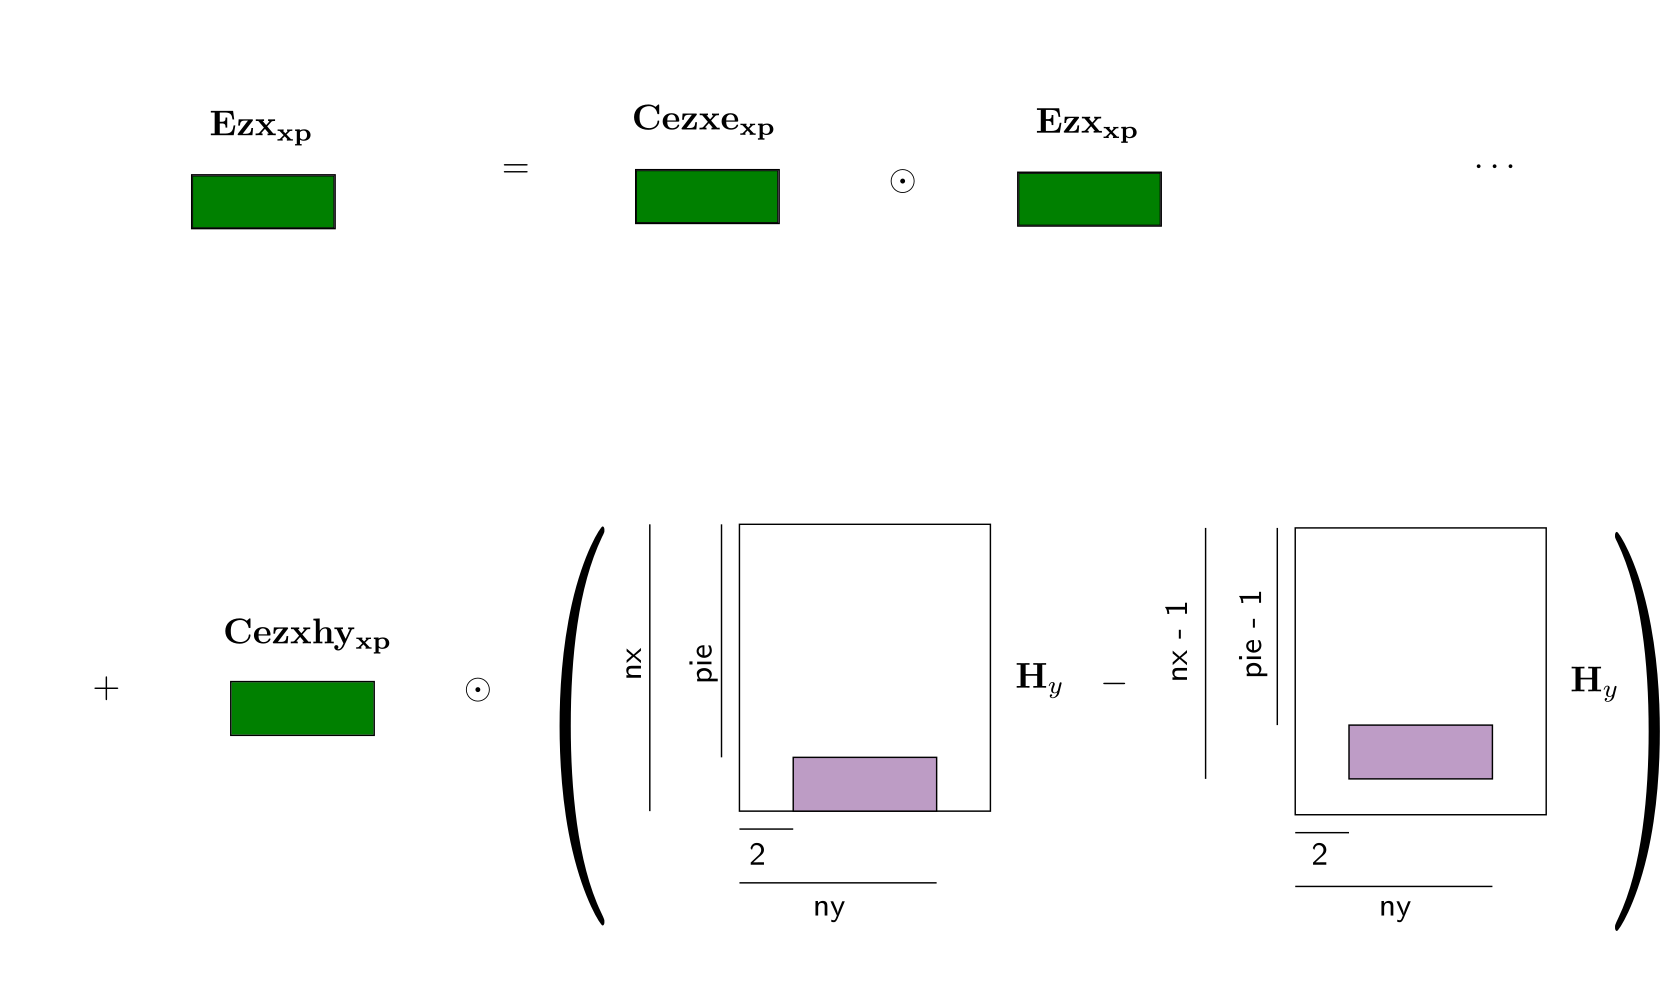
\includegraphics[width=1\textwidth]{../pics/tikz/svg/pml-color/Ezx-xp.pdf}
~
\includegraphics[width=1\textwidth]{../pics/tikz/svg/pml-color/Ezy-xp.pdf}
\caption{PML update for ${\bf E}_{zx}$ down. One line of nodes into inner nodes.}
\end{figure}
%
\begin{figure}
\centering
\includegraphics[width=1\textwidth]{../pics/tikz/svg/pml-color/Ezx-yn.pdf}
~
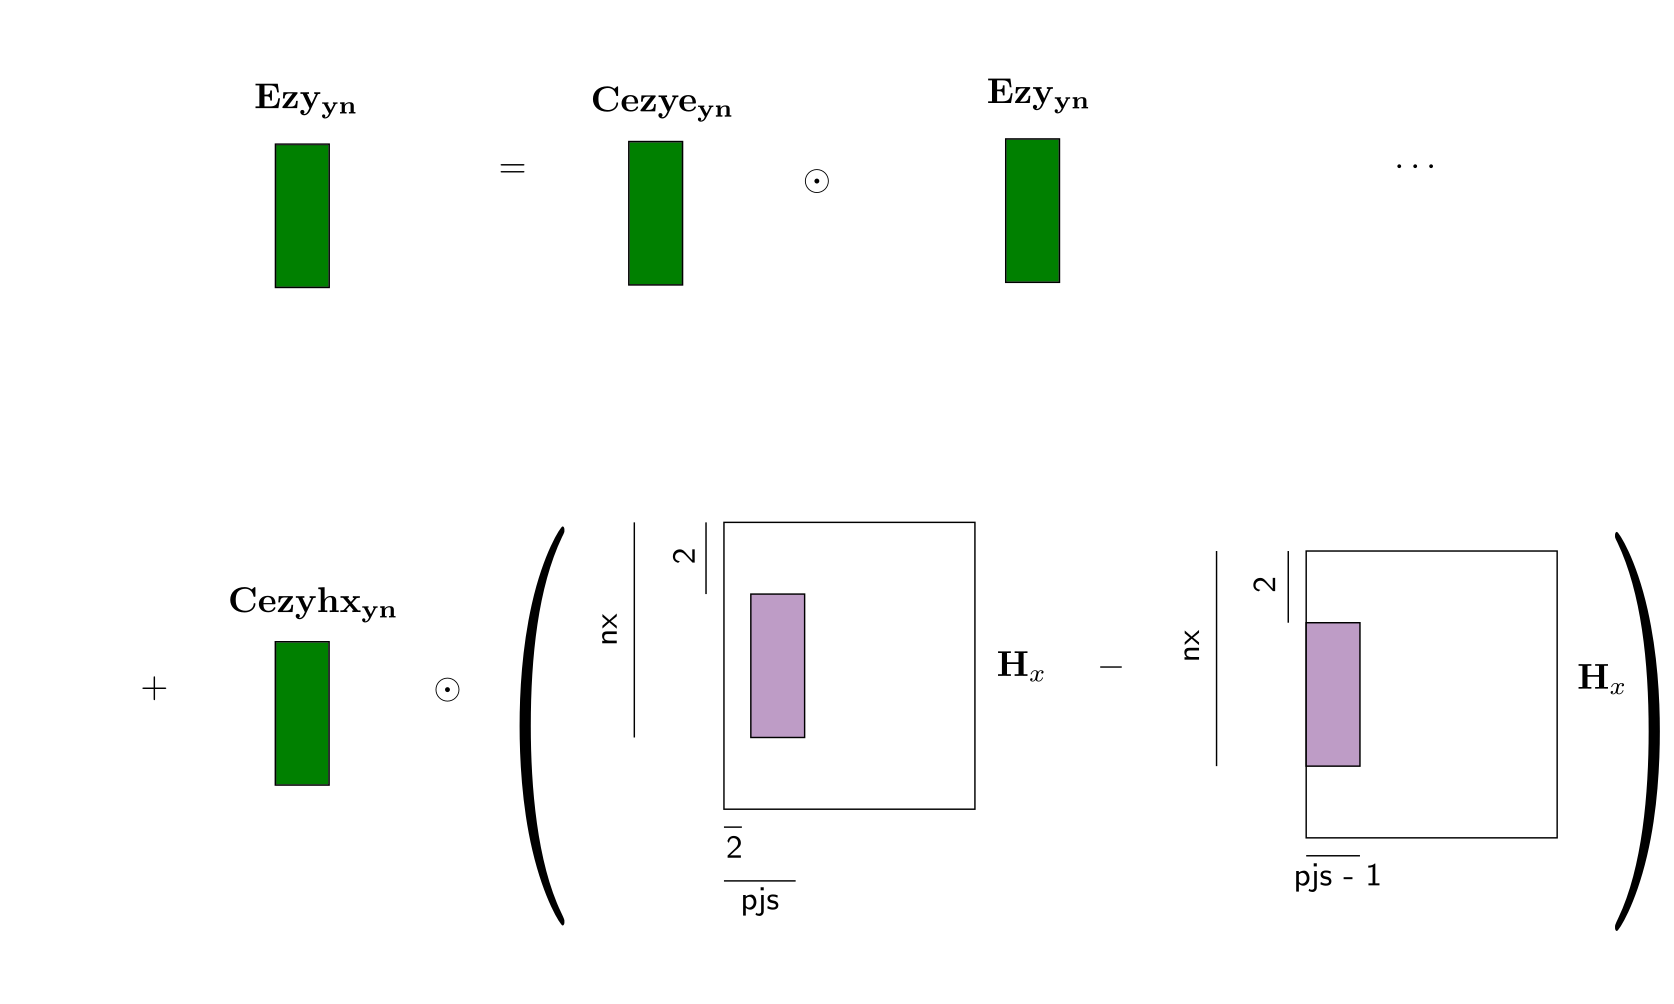
\includegraphics[width=1\textwidth]{../pics/tikz/svg/pml-color/Ezy-yn.pdf}
\caption{PML update for ${\bf E}_{zy}$ left. One line of nodes into inner nodes.}
\end{figure}
%
\begin{figure}
\centering
\includegraphics[width=1\textwidth]{../pics/tikz/svg/pml-color/Ezx-yp.pdf}
~
\includegraphics[width=1\textwidth]{../pics/tikz/svg/pml-color/Ezy-yp.pdf}
\caption{PML update for ${\bf E}_{zy}$ right. One line of nodes into inner nodes.}
\end{figure}
%
% Ez = Ezx + Ezy
%
\begin{figure}
\centering
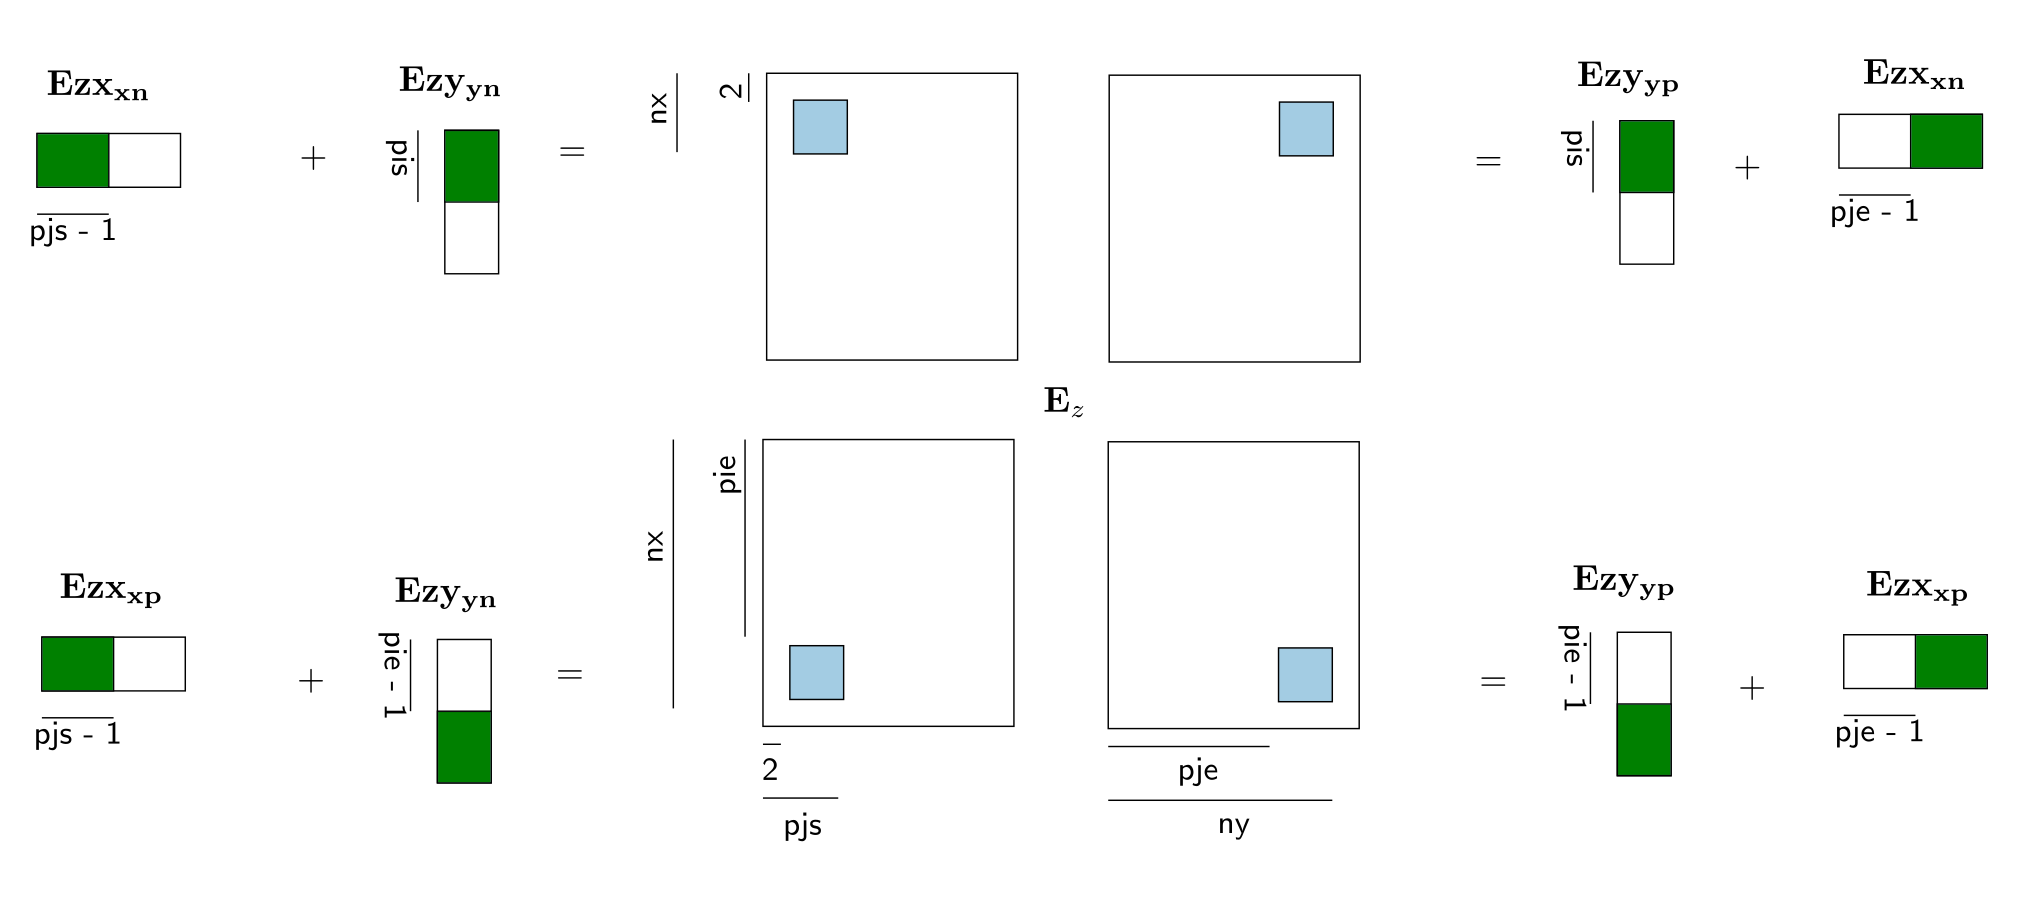
\includegraphics[width=1.4\textwidth,angle=90,origin=c]{../pics/tikz/svg/pml-color/Ex-plus-Ey.pdf}
\caption{PML update for ${\bf E}_z = {\bf E}_{zx} + {\bf E}_{zy}$ corners. PML proper.}
\end{figure}
%
\begin{figure}
\centering
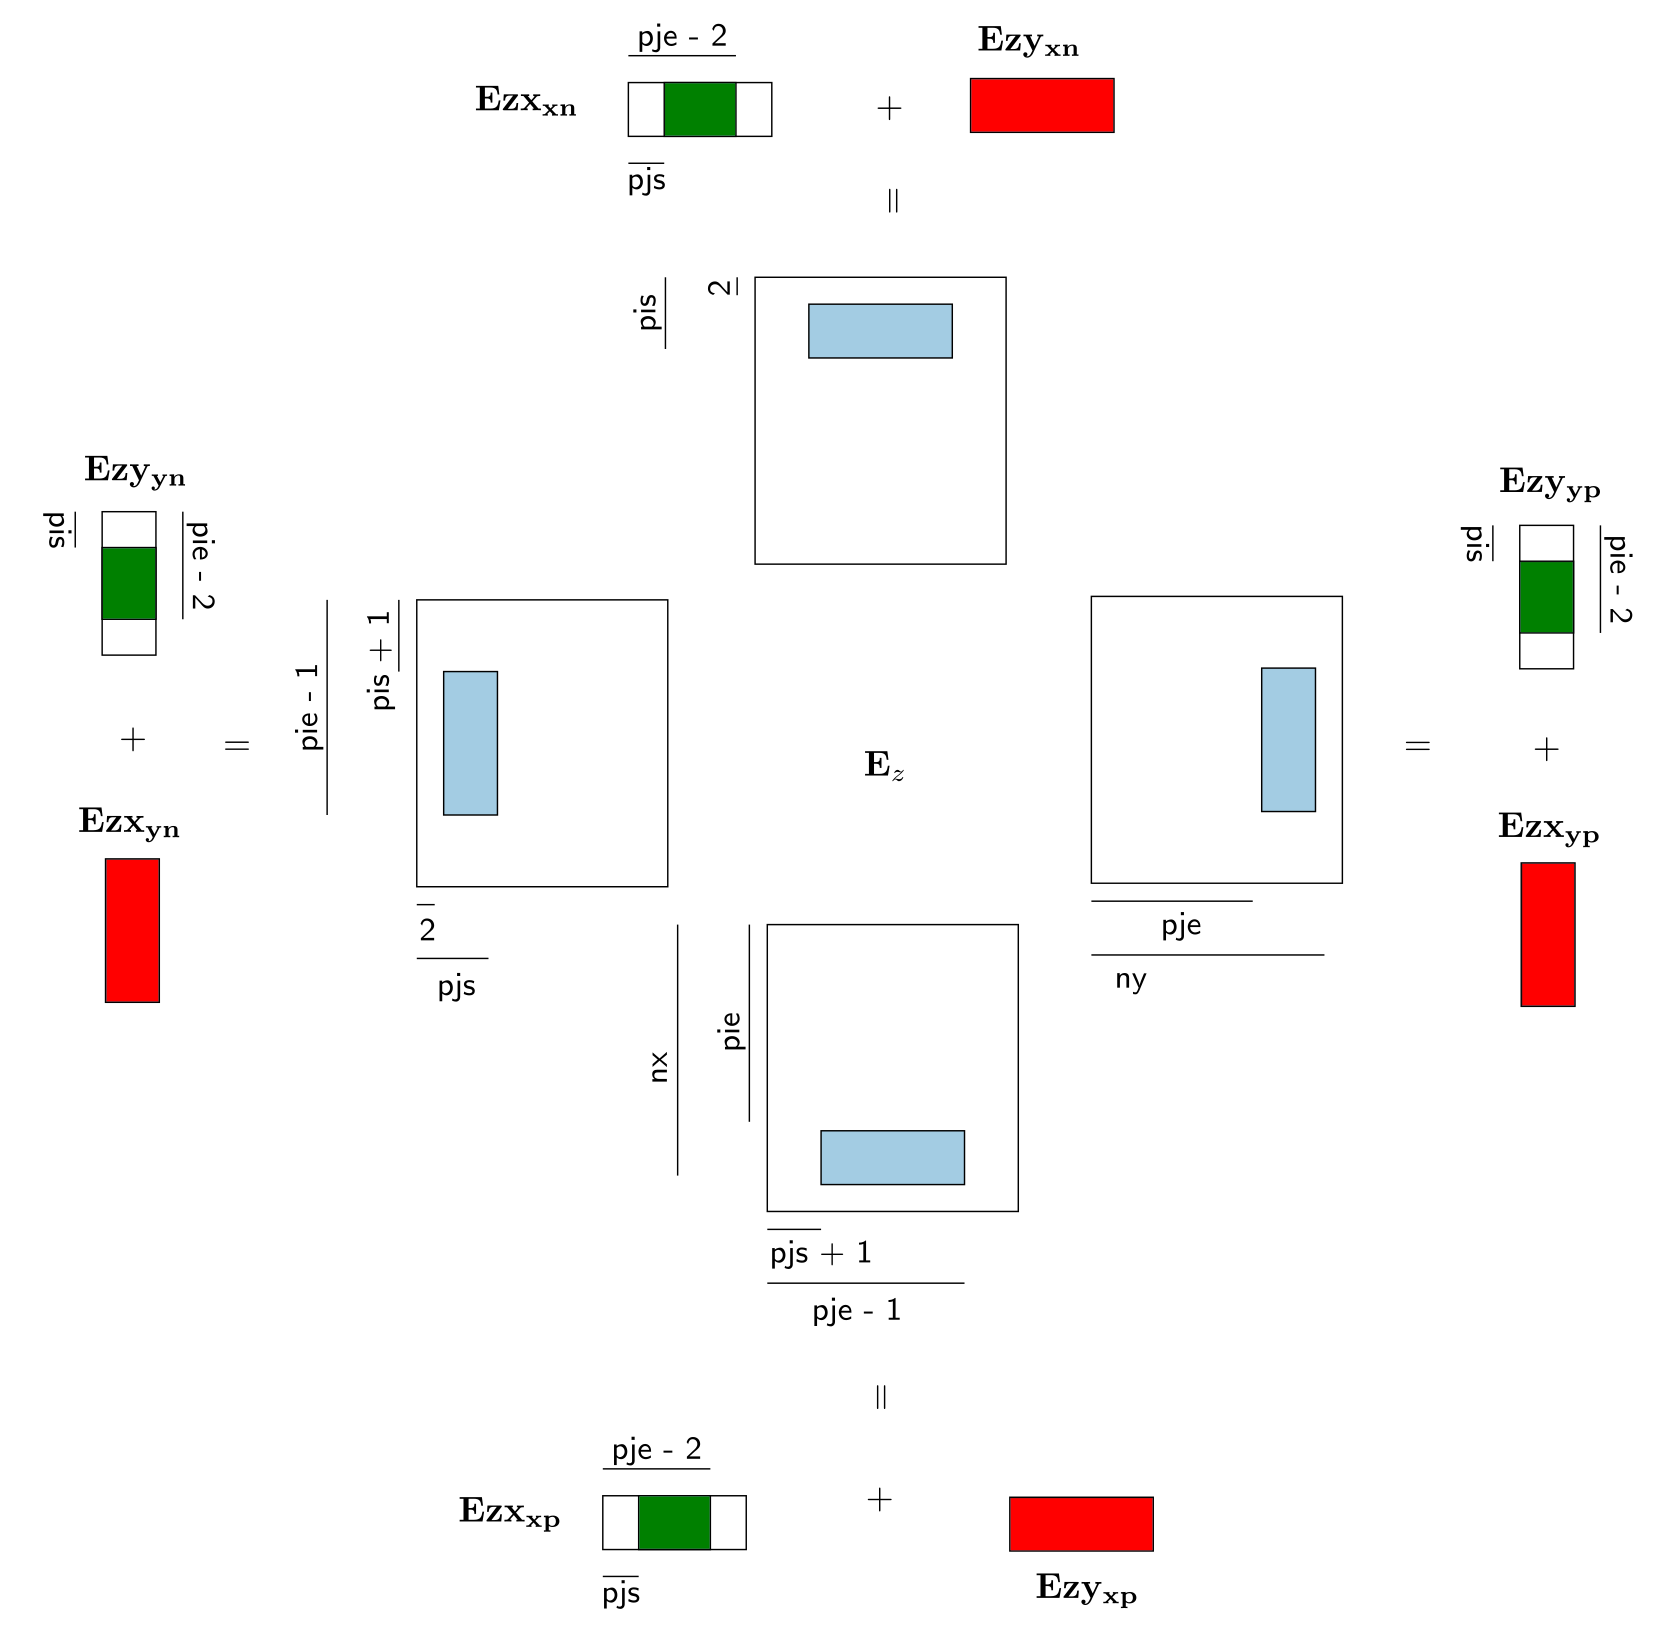
\includegraphics[width=1\textwidth]{../pics/tikz/svg/pml-color/Ex-plus-Ey-long.pdf}
\caption{PML update for ${\bf E}_z = {\bf E}_{zx} + {\bf E}_{zy}$ sides. PML proper.}
\end{figure}
%------------
% biblio
%------------
%\newpage
%\bibliographystyle{plainnat}
%\bibliography{seis-flow}
%\nocite{*}
\end{document}